\documentclass[9pt,twocolumn,twoside,]{pnas-new}

% Use the lineno option to display guide line numbers if required.
% Note that the use of elements such as single-column equations
% may affect the guide line number alignment.


\usepackage[T1]{fontenc}
\usepackage[utf8]{inputenc}

% tightlist command for lists without linebreak
\providecommand{\tightlist}{%
  \setlength{\itemsep}{0pt}\setlength{\parskip}{0pt}}


% Pandoc citation processing
\newlength{\cslhangindent}
\setlength{\cslhangindent}{1.5em}
\newlength{\csllabelwidth}
\setlength{\csllabelwidth}{3em}
\newlength{\cslentryspacingunit} % times entry-spacing
\setlength{\cslentryspacingunit}{\parskip}
% for Pandoc 2.8 to 2.10.1
\newenvironment{cslreferences}%
  {}%
  {\par}
% For Pandoc 2.11+
\newenvironment{CSLReferences}[2] % #1 hanging-ident, #2 entry spacing
 {% don't indent paragraphs
  \setlength{\parindent}{0pt}
  % turn on hanging indent if param 1 is 1
  \ifodd #1
  \let\oldpar\par
  \def\par{\hangindent=\cslhangindent\oldpar}
  \fi
  % set entry spacing
  \setlength{\parskip}{#2\cslentryspacingunit}
 }%
 {}
\usepackage{calc}
\newcommand{\CSLBlock}[1]{#1\hfill\break}
\newcommand{\CSLLeftMargin}[1]{\parbox[t]{\csllabelwidth}{#1}}
\newcommand{\CSLRightInline}[1]{\parbox[t]{\linewidth - \csllabelwidth}{#1}\break}
\newcommand{\CSLIndent}[1]{\hspace{\cslhangindent}#1}


\templatetype{pnasresearcharticle}  % Choose template

\title{Portrait de la biodiversité aviaire au Québec}

\author[a]{Émy Chevrette}
\author[a]{Angélique Cornellier}
\author[a]{Coralie Mimeault}
\author[a]{Stéphanie Morin-Beaumier}

  \affil[a]{Université de Sherbrooke, Département de biologie, 2500
Boulevard de l'Université, Sherbrooke, Québec, J1K 2R1}


% Please give the surname of the lead author for the running footer
\leadauthor{Chevrette}

% Please add here a significance statement to explain the relevance of your work
\significancestatement{}


\authorcontributions{}



\correspondingauthor{\textsuperscript{} }

% Keywords are not mandatory, but authors are strongly encouraged to provide them. If provided, please include two to five keywords, separated by the pipe symbol, e.g:
 \keywords{  Aviaire |  Biodiversité  } 

\begin{abstract}
Les suivis des dynamiques de population sont essentiels dans un objectif
de conservation des espèces d'un territoire, particulièrement à l'ère où
les pressions sur les milieux naturels sont fortes et accélèrent
l'érosion de la biodiversité. La faune aviaire, qui connait actuellement
un déclin marqué à travers le globe, est un groupe particulièrement visé
par ce type de suivi. Un programme de suivi initié en 2016 au Québec et
s'étalant sur 5 ans a permis de recenser des données de biodiversité
d'oiseaux au Québec. Leur analyse a permis de faire ressortir des
patrons temporels, spatiaux et taxonomiques. L'abondance et la richesse
spécifique s'avèrent plus élevées au mois de juin, avec une majorité
d'observations concentrées au sud du 49e parallèle.
\end{abstract}

\dates{This manuscript was compiled on \today}
\doi{\url{www.pnas.org/cgi/doi/10.1073/pnas.XXXXXXXXXX}}

\begin{document}

% Optional adjustment to line up main text (after abstract) of first page with line numbers, when using both lineno and twocolumn options.
% You should only change this length when you've finalised the article contents.
\verticaladjustment{-2pt}



\maketitle
\thispagestyle{firststyle}
\ifthenelse{\boolean{shortarticle}}{\ifthenelse{\boolean{singlecolumn}}{\abscontentformatted}{\abscontent}}{}

% If your first paragraph (i.e. with the \dropcap) contains a list environment (quote, quotation, theorem, definition, enumerate, itemize...), the line after the list may have some extra indentation. If this is the case, add \parshape=0 to the end of the list environment.

\acknow{}

\hypertarget{introduction}{%
\section{Introduction}\label{introduction}}

Dans le contexte de crise de biodiversité actuel, les données sur la
répartition et l'abondance en espèces d'un territoire fournissent de
précieuses informations sur les dynamiques de populations. Cela est
particulièrement pertinent du côté des espèces aviaires, qui subissent
les impacts de la perte d'habitats dont le rythme est en hausse
continuelle (1). L'étude de la répartition et de l'abondance d'espèces
d'oiseaux fournit une myriade d'informations sur la qualité d'un site
et, par le fait même, sur l'état des populations d'oiseaux qui s'y
trouvent. C'est dans ce contexte que l'analyse de données d'observations
d'oiseaux entre 2016 et 2020 à l'échelle de la province du Québec a été
réalisée. Plus précisément, l'objectif est de répondre à la question
suivante : qu'est-ce qui explique les différents patrons de biodiversité
d'espèces d'oiseaux observés à travers la province du Québec ? Pour ce
faire, la question sera approchée avec les points de vue temporels,
géographiques ainsi que taxonomiques.

\hypertarget{muxe9thode-et-ruxe9sultats}{%
\section{Méthode et résultats}\label{muxe9thode-et-ruxe9sultats}}

Un jeu de donnée mesurant la composition et la phénologie acoustiques
des oiseaux du Québec a été réalisé à la suite d'un programme de suivi
de la biodiversité acoustique exécuté par le Ministère de
l'Environnement, de la Lutte contre les Changements Climatiques, de la
Faune et des Parcs (MELCCFP) dans le cadre du Réseau de suivi de la
biodiversité du Québec. Ces données regroupent les observations
acoustiques d'oiseaux. Pour chaque observation, les informations
suivantes ont été récoltées : la latitude du site, l'heure de début et
de fin de l'observation, la date et l'heure de l'observation ainsi que
les informations taxonomiques reliées à l'espèce observée. Les données
ont été traitées et analysées dans le logiciel RStudio.

\begin{figure}
\centering
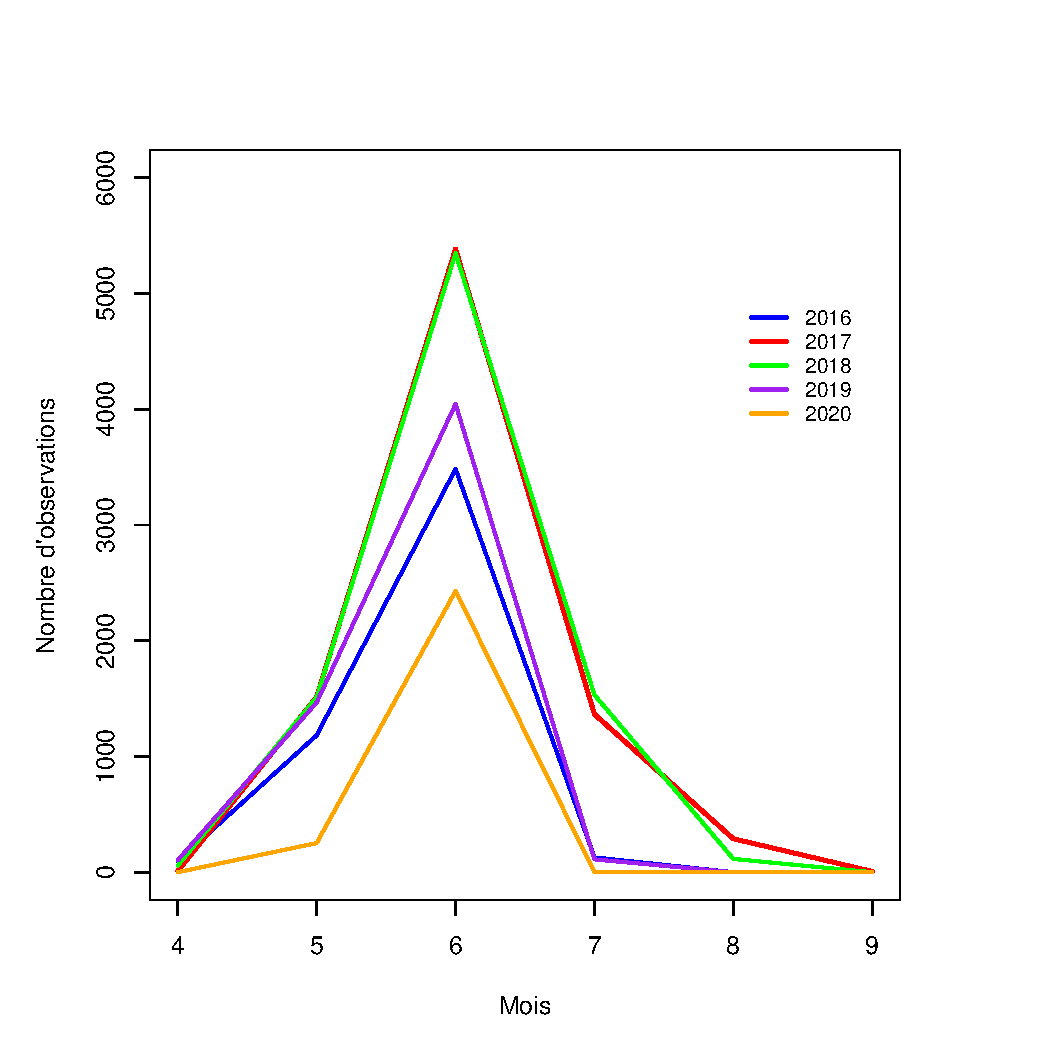
\includegraphics[width=0.5\textwidth,height=0.4\textheight]{../figures/observation_mois_annee.pdf}
\caption{Nombre d'observations d'oiseaux en fonction du mois entre 2016
et 2020\label{fig:plot1}}
\end{figure}

Un premier graphique a été réalisé illustrant le patron temporel des
observations d'oiseaux entre 2016 et 2020 (Figure \ref{fig:plot1}) .
Celui-ci met en relation le nombre d'observations, en fonction du mois,
présentés sous forme de chiffres, et ce, pour les 5 années couvrant les
données. On remarque tout d'abord que le plus grand nombre
d'observations est réalisé au 6e mois, soit le mois de juin, pour toutes
les années représentées. Le nombre d'observation débute à 0 en avril et
augmente graduellement jusqu'en juin, pour ensuite redescendre et
atteindre 0 à nouveau en septembre. Aucune observation n'a été
enregistrée entre les mois de septembre et avril.

La seconde visualisation représente l'effet de la géographie sur la
distribution des observations, obtenue au moyen d'une régression
linéaire simple intégrant le nombre d'observations en fonction de la
latitude, qui varie entre 45.00642 et 61.31273 (Figure \ref{fig:plot2}).
On remarque qu'une très grande majorité des observations ont été
réalisées sur des sites situés au sud du 50e parallèle. Très peu
d'observations proviennent de la portion nord du territoire québécois.

\begin{figure}
\centering
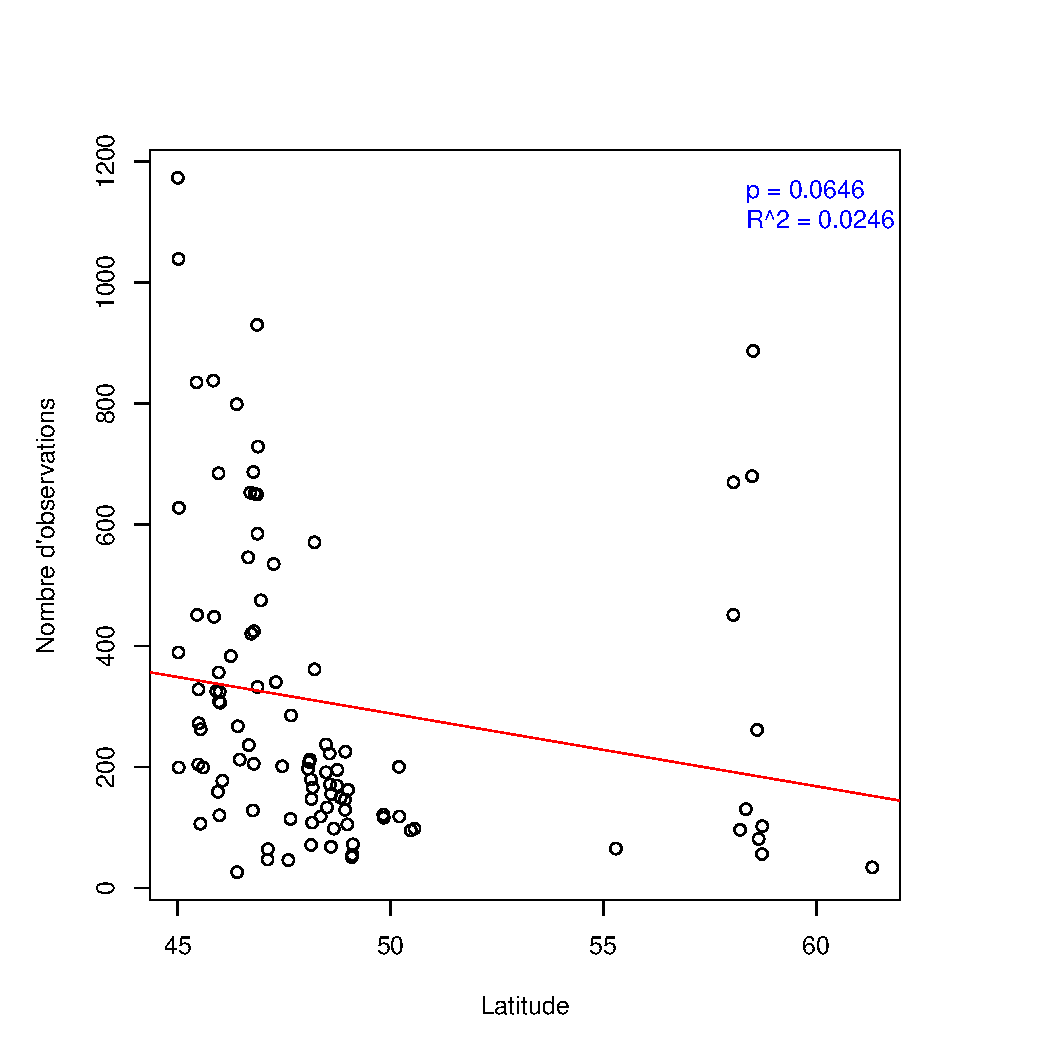
\includegraphics[width=0.5\textwidth,height=0.4\textheight]{../figures/observation_lat.pdf}
\caption{Nombre d'observations d'oiseaux en fonction de la
latitude\label{fig:plot2}}
\end{figure}

Pour compléter le portrait de la distribution de la biodiversité, un
troisième graphique intégrant les informations taxonomiques des
observations a été réalisé(Figure \ref{fig:plot3}). Celui-ci illustre le
nombre de familles recensées pour chaque mois ayant fait l'objet du
suivi, et ce, pour les 5 années du projet. Pour chacune des années, le
nombre de familles semble suivre une distribution normale, avec un
maximum atteint chaque année au mois de juin.

\hypertarget{discussion}{%
\section{Discussion}\label{discussion}}

\hypertarget{distribution-temporelle-et-taxonomique}{%
\paragraph{3.1 Distribution temporelle et
taxonomique}\label{distribution-temporelle-et-taxonomique}}

\hfill\break
Les patrons de distribution du nombre d'observations au fil des mois
témoignent directement du phénomène de migration observé au printemps et
à l'automne sur le territoire québécois. Les mouvements migratoires
débutent généralement au mois de mars, et augmentent en intensité
jusqu'en juin. À ce moment, toutes les espèces d'oiseaux qui passeront
l'été au Québec sont arrivées sur le territoire, ce qui correspond au
pic d'observations observables sur le premier graphique. Par la suite,
vers le mois d'août, c'est la migration automnale qui débute, et
graduellement les espèces migratrices quittent le territoire. Les
mouvements migratoires expliqueraient donc la variation dans le nombre
d'observations, mais serait aussi à l'origine de la distribution du
nombre de familles recensées au fil des mois représentée dans le
troisième graphique. L'abondance de familles observées qui atteint son
apogée en juin serait entre autres expliquées par l'arrivée des
passereaux migratoires, un groupe très diversifié, au cours du mois de
mai (2).

\begin{figure}
\centering
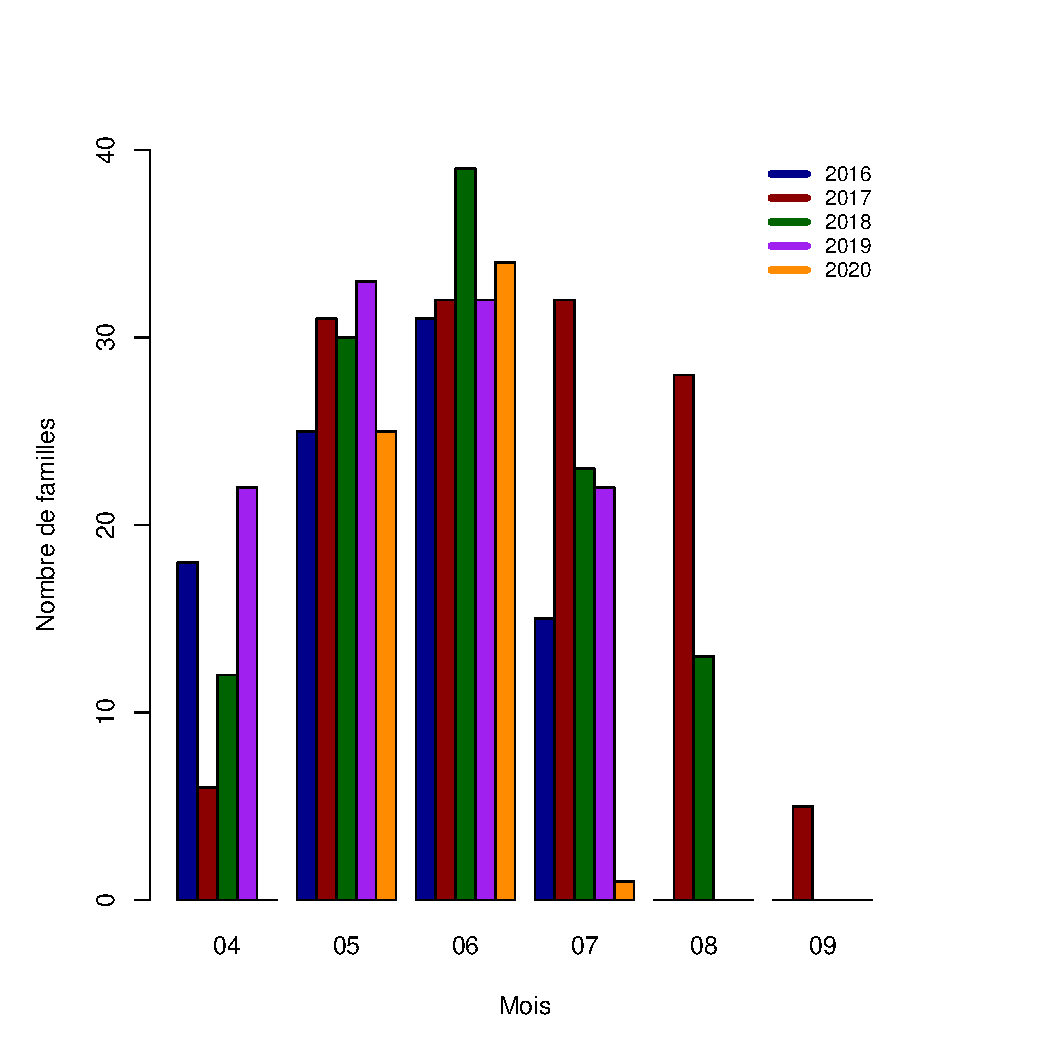
\includegraphics[width=0.5\textwidth,height=0.35\textheight]{../figures/observation_mois_famille.pdf}
\caption{Nombre de familles d'oiseaux en fonction du mois entre 2016 et
2020\label{fig:plot3}}
\end{figure}

\hypertarget{distribution-spatiale}{%
\paragraph{3.2 Distribution spatiale}\label{distribution-spatiale}}

\hfill\break
L'abondance nettement plus marquée du côté des basses-terres du
Saint-Laurent pourrait s'expliquer par le fait que cette portion de la
province, constituée majoritairement de forêt tempérée, présente
plusieurs types de domaines bioclimatiques (3). La grande diversité
d'écosystèmes qui s'y trouve, parmi lesquels se trouvent des milieux
forestiers, des milieux humides et aquatiques ainsi que des friches et
prairies agricoles, offre ainsi un habitat à davantage d'espèces (4). Le
nord du Québec est quant à lui dominé par la forêt boréale et
caractérisé par un climat plus hostile (3), qui sont deux éléments
pouvant expliquer la plus faible abondance d'oiseaux recensés.
Toutefois, il est également possible qu'il y ait un biais provenant de
l'effort d'échantillonnage déployé. En effet, si les ressources humaines
sont moins accessibles au nord pour réaliser les inventaires, cela se
reflète donc sur le nombre d'observations et pourrait mener à une
sous-estimation de la biodiversité qui se trouve sur ces sites. Ce biais
peut également se refléter dans les données du sud du Québec par une
sur-estimation. En effet, si les observateurs sont très nombreux sur un
même site, il se pourrait qu'un même oiseau face l'objet de plusieurs
observations distinctes dans la base de données.

\hypertarget{bibliographie}{%
\section*{Bibliographie}\label{bibliographie}}
\addcontentsline{toc}{section}{Bibliographie}

\hypertarget{refs}{}
\begin{CSLReferences}{0}{0}
\leavevmode\vadjust pre{\hypertarget{ref-betts_forest_2022}{}}%
\CSLLeftMargin{1. }%
\CSLRightInline{M. G. Betts, \emph{et al.},
\href{https://doi.org/10.1038/s41559-022-01737-8}{Forest degradation
drives widespread avian habitat and population declines}. \emph{Nature
Ecology \& Evolution} \textbf{6}, 709--719 (2022).}

\leavevmode\vadjust pre{\hypertarget{ref-desrochers_programme_2017}{}}%
\CSLLeftMargin{2. }%
\CSLRightInline{A. Desrochers, B. Drolet,
\href{https://doi.org/10.7202/1039737ar}{Le {Programme} de surveillance
des oiseaux nicheurs de la {Forêt} {Montmorency} : Une nouvelle source
de tendances des populations d'oiseaux nicheurs pour la forêt boréale au
{Québec}}. \emph{Le Naturaliste canadien} \textbf{141}, 61--74 (2017).}

\leavevmode\vadjust pre{\hypertarget{ref-tardif_atlas_2005}{}}%
\CSLLeftMargin{3. }%
\CSLRightInline{B. Tardif, G. Lavoie, Y. Lachance,
\emph{\href{https://belsp.uqtr.ca/id/eprint/1230/1/Tardif\%20et\%20al_2005_Esp\%C3\%A8ces_menac\%C3\%A9es_vuln\%C3\%A9rables.pdf}{Atlas
de la biodiversité du {Québec}}} (Gouvernement du Québec, ministère du
Développement durable, de l'Environnement et des Parcs, Direction du
développement durable, du patrimoine écologique et des parcs, 2005).}

\leavevmode\vadjust pre{\hypertarget{ref-jobin_latlas_2020}{}}%
\CSLLeftMargin{4. }%
\CSLRightInline{B. Jobin, \emph{et al.},
\href{https://doi.org/10.7202/1073990ar}{L'atlas des territoires
d'intérêt pour la conservation dans les basses-terres du
{Saint}-{Laurent} : Un outil pour orienter la conservation des milieux
naturels dans le sud du {Québec}}. \emph{Le Naturaliste canadien}
\textbf{144}, 47--64 (2020).}

\end{CSLReferences}



% Bibliography
% \bibliography{pnas-sample}

\end{document}
